\section {Algoritmo e Flowchart}
\hypertarget{section::\theHsection}
In questo capitolo descriveremo i passi dell'algoritmo sviluppato. Essendo l'interazione complessa si è scelto di utilizzare un diagramma di flusso per dare una visione generale di più immediata comprensione.
Il flowchart completo di tutto l'algoritmo è mostrato in Figura 8.1

\begin{figure}[htp]
\centering
{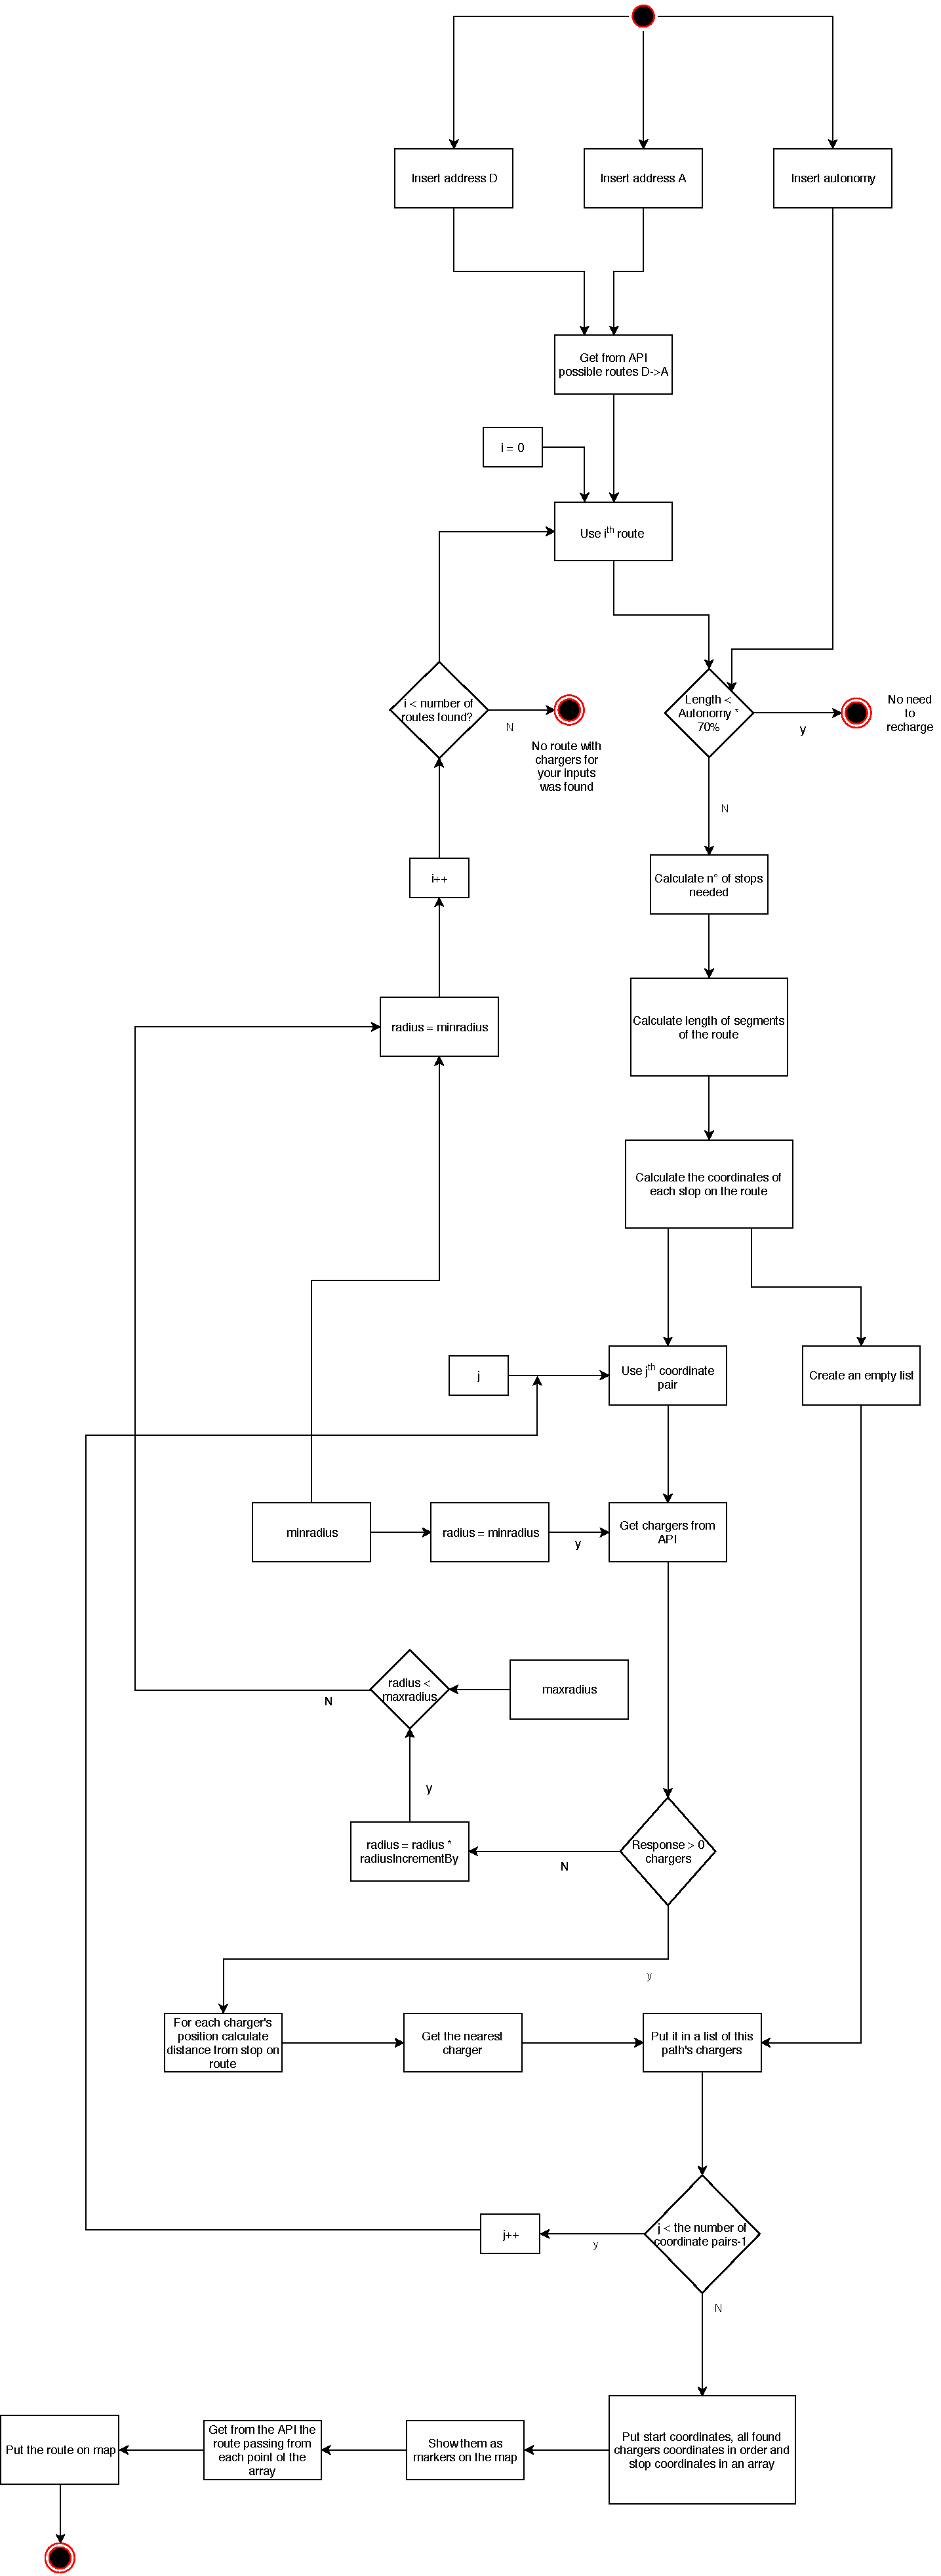
\includegraphics[scale=0.30]{Immagini/Algoritmo_Flowchart.pdf}}
\caption{Flowchart Algorithm}
\end{figure}

\subsection{Analisi di complessità}
\hypertarget{section::\theHsection}
Procediamo ora all'analisi di complessità dell'algoritmo. Per cercare di analizzarlo risulta utile avere un'idea più chiara e di alto livello su ciò che l'algoritmo effettivamente fa; una spiegazione testuale può quindi risultare utile.
L'esecuzione inizia richiedendo a OpenStreetMap il percorso fra il punto di partenza e il punto di arrivo inseriti dall'utente. L'API restituisce tutti i percorsi che è riuscita a trovare in ordine ottimale, ossia in ordine crescente di tempo di percorrenza. E' importante notare, per il proseguo della spiegazione, che i percorsi vengono forniti come una serie di punti adiacenti. A questo punto subentra l'algoritmo vero e proprio che analizza i percorsi nell'ordine in cui gli sono stati forniti, attraverso la funzione \textit{getStopCircleCenterPoints}, nel seguente modo: partendo dal punto iniziale si sommano le distanze (che vanno calcolate), fra i punti che costituiscono il percorso fino a raggiungere una distanza maggiore dell'autonomia dichiarata dall'utente. A questo punto si torna indietro di un punto e lo si aggiunge all'array di punti dove sarà necessario fermarsi. Alla fine di quest'analisi si ha quindi la lista delle coordinate nei pressi delle quali è necessario fermarsi. Viene quindi chiamata la funzione \textit{obtainChargersForThisRoute} la quale, insieme alla funzione \textit{getSmallestElementsIndex}, trova il charger più vicino. La ricerca del charger avviene nel seguente modo: viene definito un cerchio di raggio 1 centrato nel punto trovato in precedenza e si cerca in quest'area il charger più vicino. Nel caso non venisse trovato alcun charger si estende incrementalmente il raggio del cerchio fino ad un massimo di \[maxRadius = \frac{1 - batteryPercentageUsage}{2} * Autonomia\] Le coordinate del charger trovato vengono inserite nel percorso e questo viene conseguentemente modificato per includere il passaggio per la colonnina di ricarica. Nel caso in cui non sia possibile trovare un charger per anche solo uno dei punti in cui è necessario fermarsi, il percorso viene dichiarato invalido e l'algoritmo procede ad esaminare il successivo risultato fornitogli dall'API.
E' quindi possibile notare che l'algoritmo è costituito da una prima parte di programmazione dinamica, in cui si calcola la somma delle distanze fra tutti i punti successivi, e una seconda parte di stampo greedy, in cui si cerca la soluzione (charger) ottima più vicina, allargando mano a mano l'insieme dei candidati non ancora esplorati. \autocite[\protect\label{BertossiMontresor2000}][]{BertossiMontresor2000}

E' ora possibile analizzare la complessità dell'algoritmo: la parte dinamica si basa sulla somma degli n segmenti che costituiscono il percorso, e può quindi essere portata a termine in tempo $O(n)$.
La seconda parte greedy viene eseguita nel seguente modo: l'algoritmo riceve la lista dei charger presenti nell'area e calcola la distanza di ciascuno di essi dal centro del cerchio, quindi seleziona il charger con distanza minore. Dato \textit{m} il numero di charger restituiti dall'API per quell'area, l'operazione è semplicemente il calcolo della distanza e viene quindi espletata in tempo $O(m)$. Siccome il numero di charger restituiti è generalmente piccolo, l'operazione può essere eseguita in un tempo costante $\Theta(1)$. Si nota inoltre che la funzione per trovare i charger viene chiamata un numero costante di volte (molto inferiore a n), quindi l'intera operazione è $\Theta(1)$. Da ciò ne deriva che il tempo totale di esecuzione dell'algoritmo è dato solo dalla parte di calcolo delle somme delle distanze ed è perciò $O(n)$.

\subsection{Pseudocodice}
\hypertarget{section::\theHsection}
Segue lo pseudocodice.

\lstinputlisting[language=JavaScript]{Codice/pseudocode_importLibraries.pseudo}

\lstinputlisting[language=JavaScript]{Codice/pseudocode_data.pseudo}

\lstinputlisting[language=JavaScript]{Codice/pseudocode_main.pseudo}

\lstinputlisting[language=JavaScript]{Codice/pseudocode_handleRoutesFound.pseudo}

\lstinputlisting[language=JavaScript]{Codice/pseudocode_obtainChargersForThisRoute.pseudo}

\lstinputlisting[language=JavaScript]{Codice/pseudocode_calculateDistancesFromRouteCoordinates.pseudo}

\lstinputlisting[language=JavaScript]{Codice/pseudocode_getStopCircleCenterPoints.pseudo}

\lstinputlisting[language=JavaScript]{Codice/pseudocode_getSmallestElementsIndex.pseudo}

\lstinputlisting[language=JavaScript]{Codice/pseudocode_displayResults.pseudo}

\subsection{Diagrammi di attività}
\hypertarget{section::\theHsection}
Il diagramma di sequenza è mostrato in Figura 8.2 questo diagramma mostra come le varie componenti interagiscono tra di loro e i dati che si scambiano.


\begin{figure}[H]
\centering
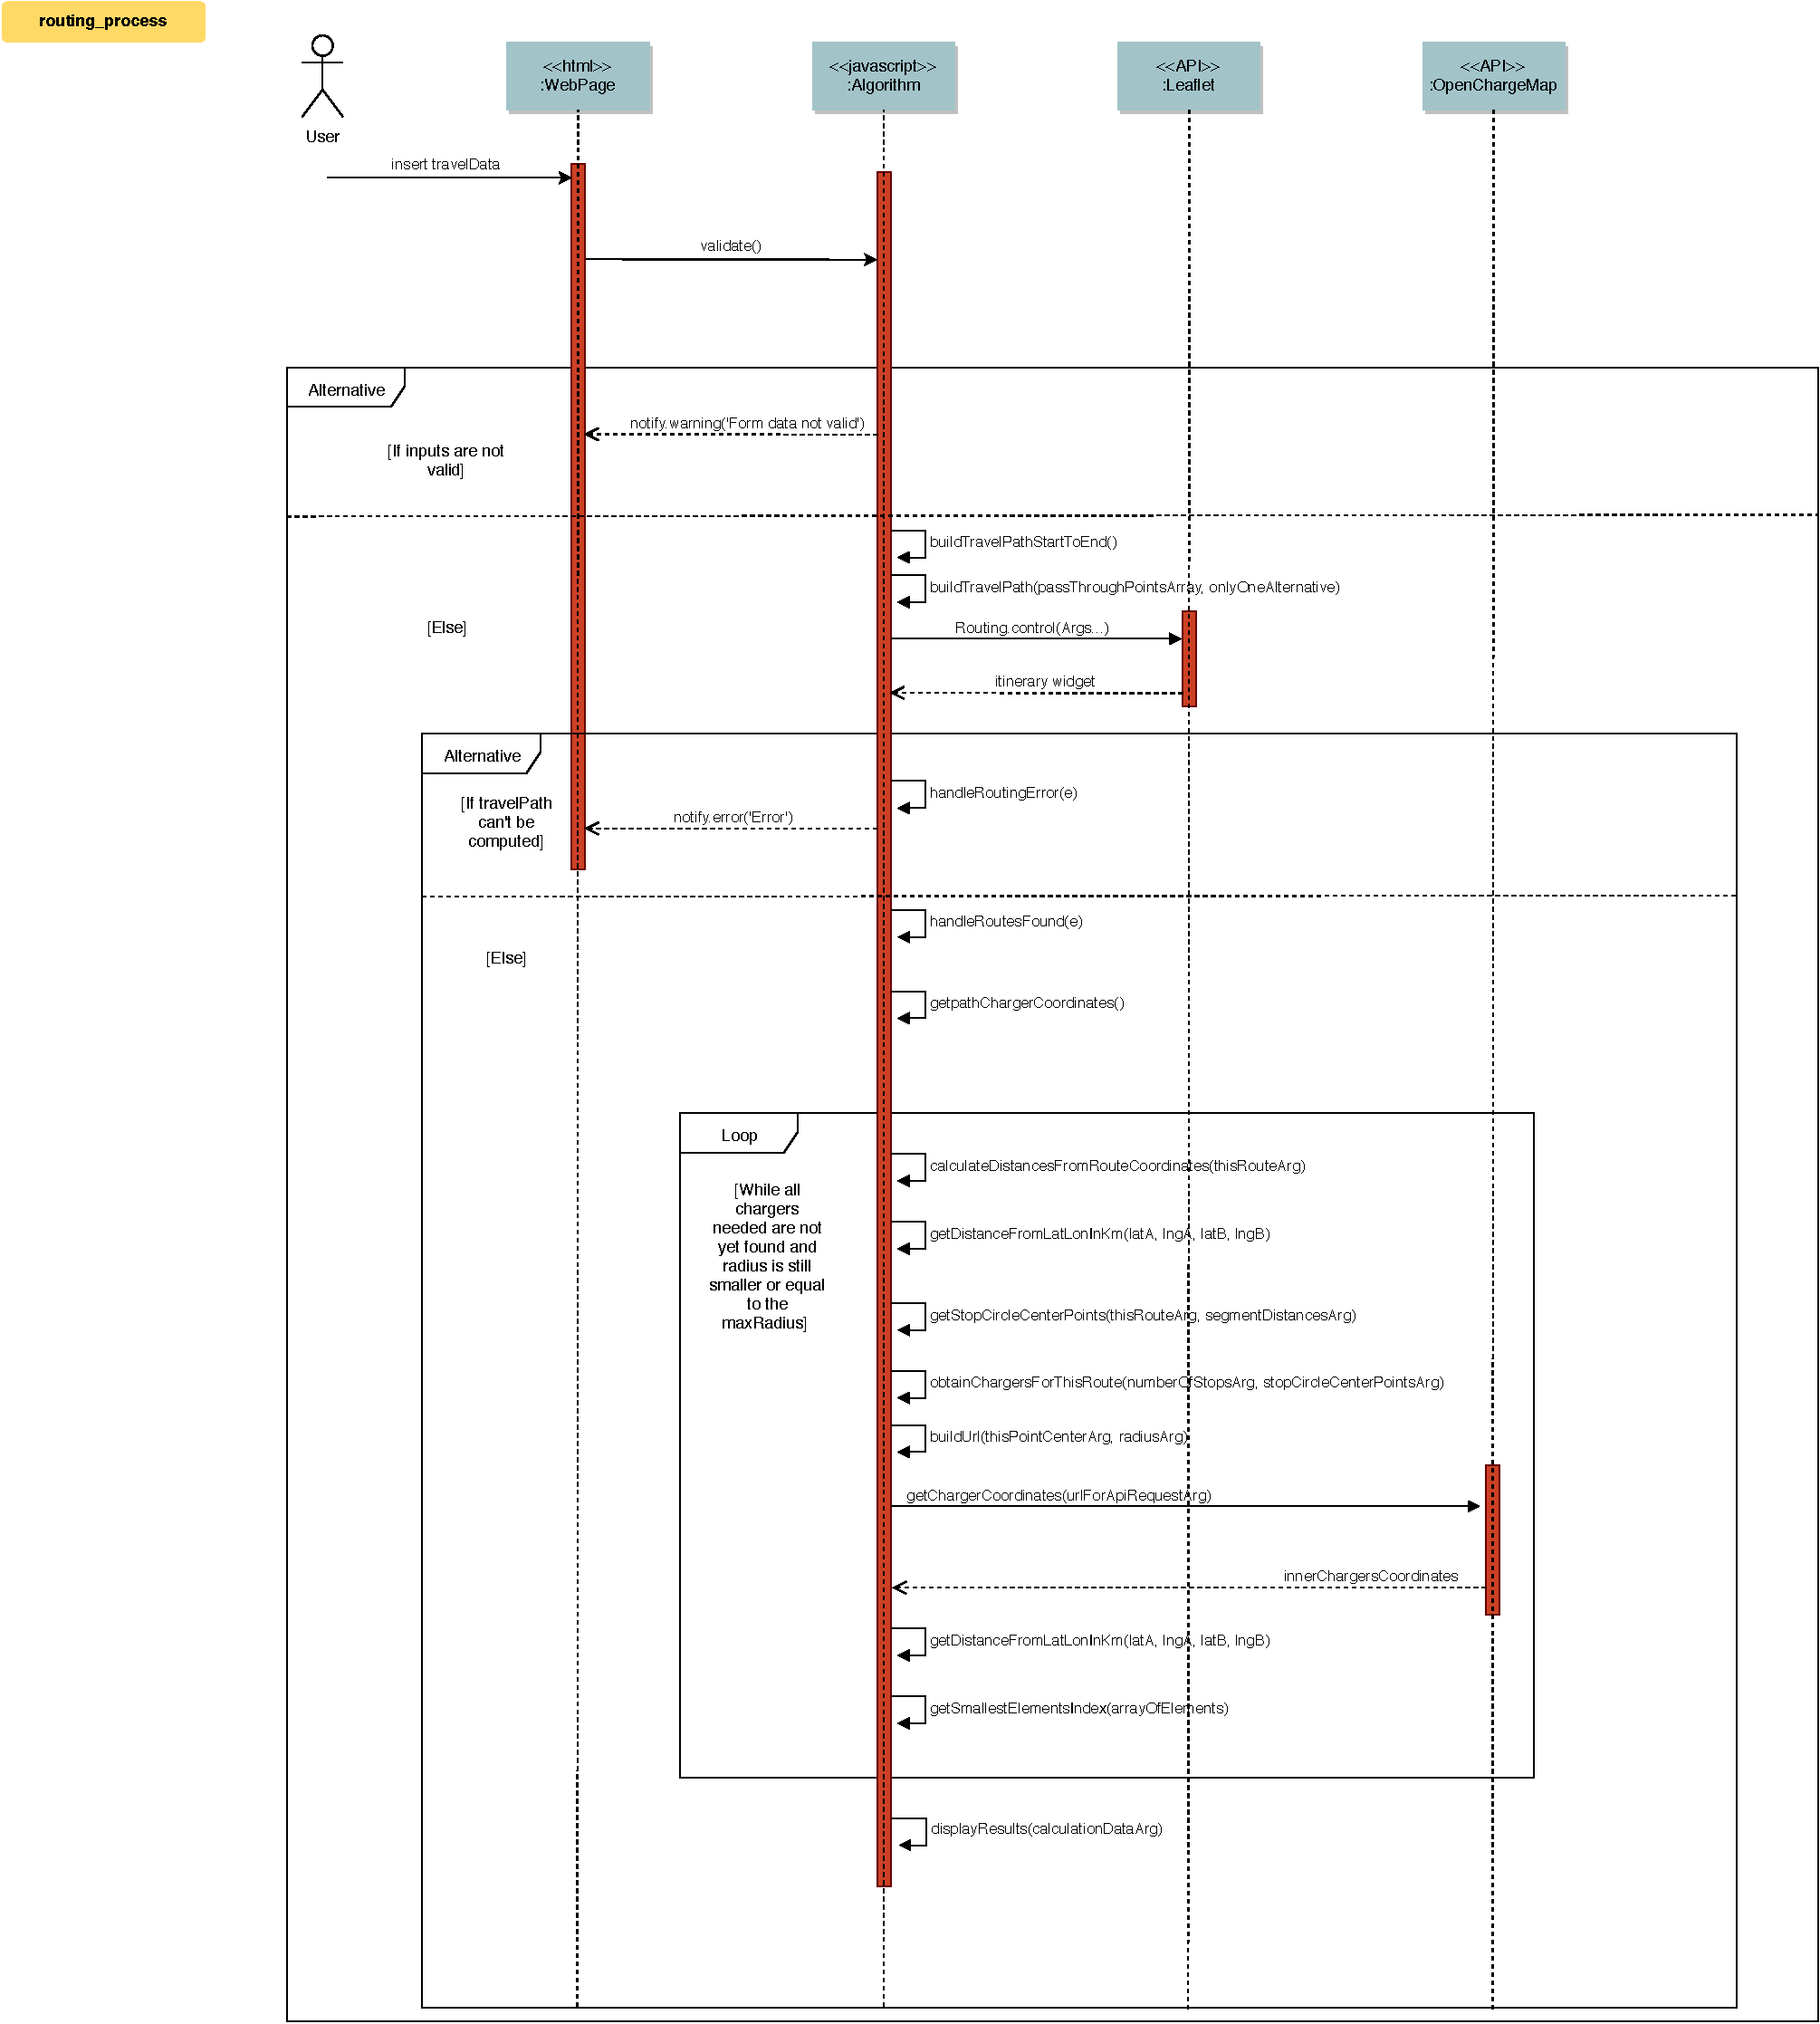
\includegraphics[scale=0.4]{Immagini/Algorithm_SequenceDiagram.pdf}
\caption{Algorithm Sequence Diagram}
\end{figure}

Nella Figura 8.3 sono mostrati, più in dettaglio, i metodi e le relative chiamate che l'algoritmo utilizza per la sua computazione.

\begin{figure}[htp]
\centering
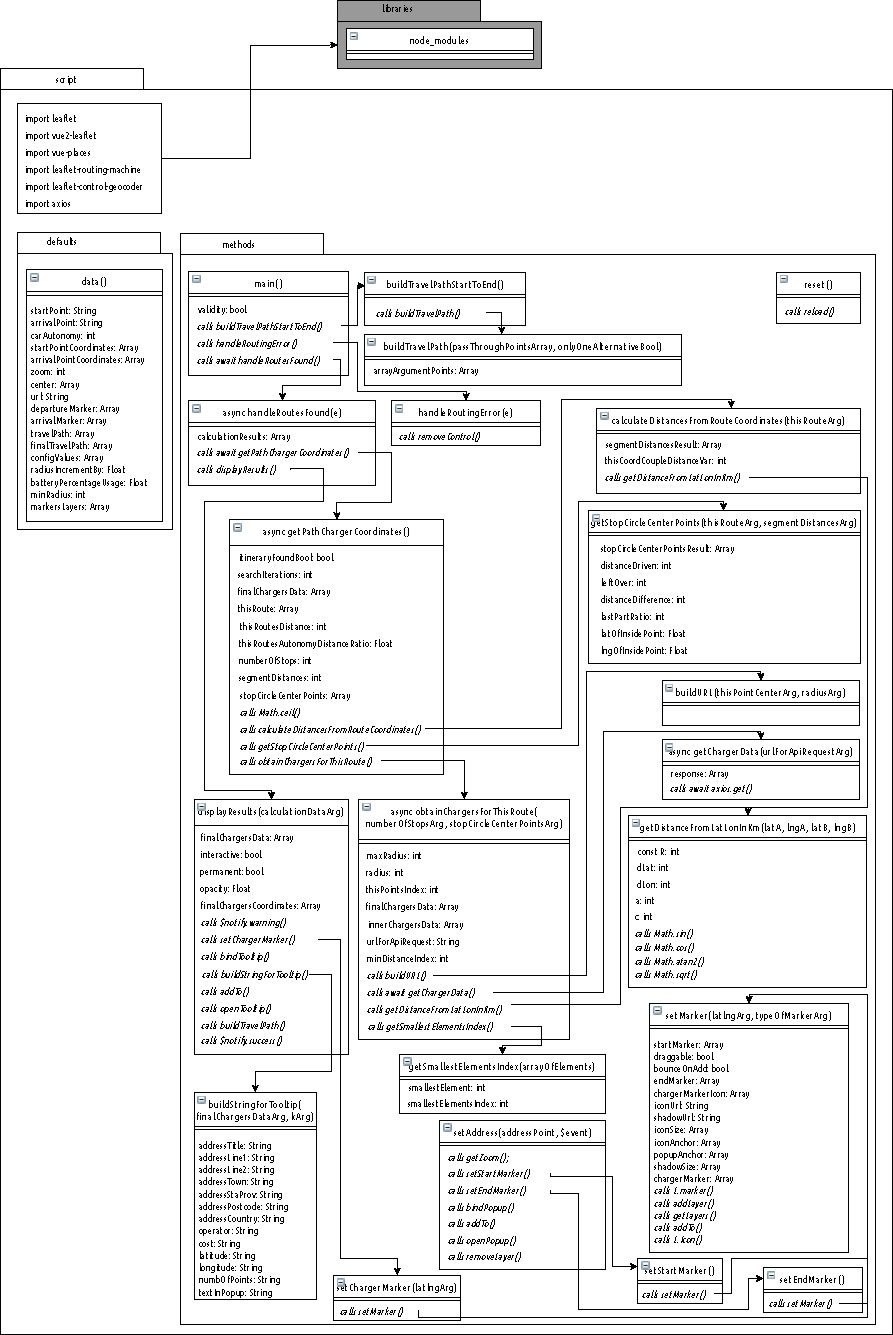
\includegraphics[scale=0.9]{Immagini/Methods_Diagram.pdf}
\caption{Methods}
\end{figure}

\section{Progettazione dei Test} 
\hypertarget{section::\theHsection}
L'algoritmo che abbiamo progettato è costituito da diverse funzioni. Per verificarne il comportamento testeremo queste funzioni controllando che i parametri passati e i valori restituiti coincidano con quanto ci aspettiamo. In particolare testeremo le funzioni riportate in tabella 8.1 .

\begin{table}[h]
\centering
\begin{tabular}{|c|l|c|}
\hline
Funzione                  & Descrizione                                                                                                                                      & Esito test \\ \hline
setMarker                 & aggiunge un Marker alla lista                                                                                                                    & Passato    \\ \hline
setChargerMarker          & aggiunge un Marker per un charger                                                                                                                & Passato    \\ \hline
setStartMarker            & aggiunge il Marker per il punto di partenza                                                                                                      & Passato    \\ \hline
setEndMarker              & aggiunge il Marker per il punto di arrivo                                                                                                        & Passato    \\ \hline
buildStringForTooltip     & \begin{tabular}[c]{@{}l@{}}costruisce la stringa da visualizzare a schermo \\ riportante le informazioni circa il punto di ricarica\end{tabular} & Passato    \\ \hline
getSmallestElementsIndex  & ottiene l'indice del charger più vicino al punto selezionato                                                                                     & Passato    \\ \hline
buildUrl                  & \begin{tabular}[c]{@{}l@{}}costruisce l'URL per effettuare la richiesta all'API \\ di Open Charge Map\end{tabular}                               & Passato    \\ \hline
getStopCircleCenterPoints & \begin{tabular}[c]{@{}l@{}}calcola il punto lungo il tragitto in cui è necessario\\  fermarsi per la ricarica\end{tabular}                       & Passato    \\ \hline
getDistanceFromLatLonInKm & calcola la distanza fra due punti                                                                                                                & Passato    \\ \hline
\end{tabular}
\caption{Funzioni implementate nella suite di test}
\end{table}


\section{Risultato dei Test} 
\hypertarget{section::\theHsection}
Il risultato dei test eseguiti è riportato nella figura qui sotto. E' stata eseguita una suite composta di nove test che hanno ricevuto esito positivo.

\begin{figure}[htp]
\centering
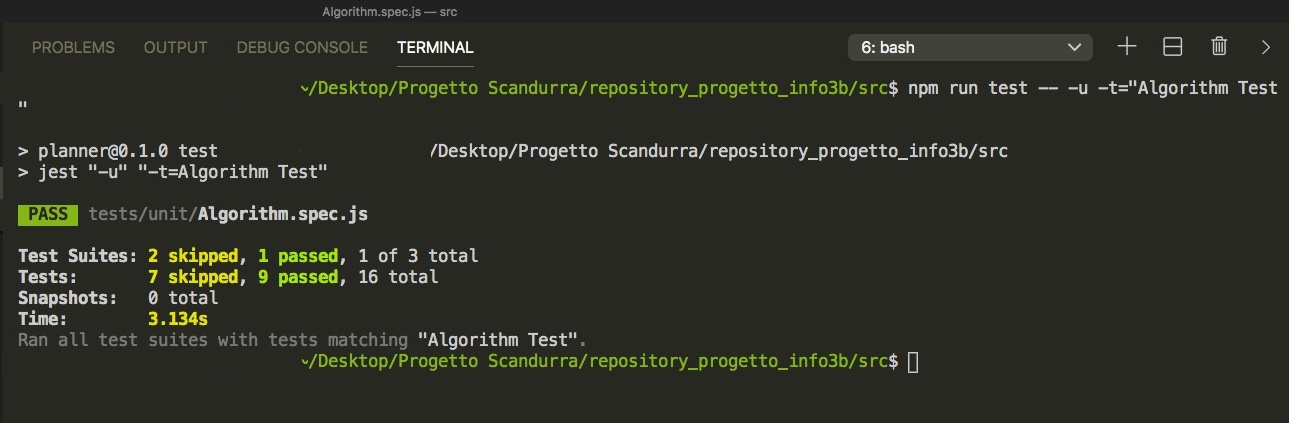
\includegraphics[scale=1.3]{Immagini/TestAlgorithm.jpeg}
\caption{Test iterazione 3}
\end{figure}

E' quindi possibile passare all'ultima iterazione del nostro processo AMDD.